% Created 2019-06-26 Wed 03:41
% Intended LaTeX compiler: pdflatex
\documentclass[12pt]{article}
\usepackage[utf8]{inputenc}
\usepackage[T1]{fontenc}
\usepackage{graphicx}
\usepackage{grffile}
\usepackage{longtable}
\usepackage{wrapfig}
\usepackage{rotating}
\usepackage[normalem]{ulem}
\usepackage{amsmath}
\usepackage{textcomp}
\usepackage{amssymb}
\usepackage{capt-of}
\usepackage{hyperref}
\author{Heitor Lourenço Werneck \\{\href{mailto:heitorwerneck@hotmail.com}{heitorwerneck@hotmail.com}}}
\usepackage[portuguese]{babel}
\usepackage{mathtools}
\usepackage[binary-units=true]{siunitx}
\usepackage[top=0.5cm,bottom=1.5cm,left=2cm,right=2cm]{geometry}
\usepackage{mdframed}
\usepackage{listings}
\usepackage[noend]{algpseudocode}
\usepackage{algorithm}
\usepackage{color}
\usepackage{tikz}
\date{\today}
\title{Arquitetura e Organização de Computadores I\\\medskip
\large Trabalho prático 2}
\hypersetup{
 pdfauthor={Heitor Lourenço Werneck},
 pdftitle={Arquitetura e Organização de Computadores I},
 pdfkeywords={},
 pdfsubject={},
 pdfcreator={Emacs 26.2 (Org mode 9.1.9)}, 
 pdflang={Portuguese}}
\begin{document}

\maketitle

\lstdefinelanguage{mips}{%
  % so listings can detect directives and register names
  alsoletter={.\$},
  % strings, characters, and comments
  morestring=[b]",
  morestring=[b]',
  morecomment=[l]\#,
  % instructions
  morekeywords={[1]abs,abs.d,abs.s,add,add.d,add.s,addi,addiu,addu,%
    and,andi,b,bc1f,bc1t,beq,beqz,bge,bgeu,bgez,bgezal,bgt,bgtu,%
    bgtz,ble,bleu,blez,blt,bltu,bltz,bltzal,bne,bnez,break,c.eq.d,%
    c.eq.s,c.le.d,c.le.s,c.lt.d,c.lt.s,ceil.w.d,ceil.w.s,clo,clz,%
    cvt.d.s,cvt.d.w,cvt.s.d,cvt.s.w,cvt.w.d,cvt.w.s,div,div.d,div.s,%
    divu,eret,floor.w.d,floor.w.s,j,jal,jalr,jr,l.d,l.s,la,lb,lbu,%
    ld,ldc1,lh,lhu,li,ll,lui,lw,lwc1,lwl,lwr,madd,maddu,mfc0,mfc1,%
    mfc1.d,mfhi,mflo,mov.d,mov.s,move,movf,movf.d,movf.s,movn,movn.d,%
    movn.s,movt,movt.d,movt.s,movz,movz.d,movz.s,msub,msubu,mtc0,mtc1,%
    mtc1.d,mthi,mtlo,mul,mul.d,mul.s,mulo,mulou,mult,multu,mulu,neg,%
    neg.d,neg.s,negu,nop,nor,not,or,ori,rem,remu,rol,ror,round.w.d,%
    round.w.s,s.d,s.s,sb,sc,sd,sdc1,seq,sge,sgeu,sgt,sgtu,sh,sle,%
    sleu,sll,sllv,slt,slti,sltiu,sltu,sne,sqrt.d,sqrt.s,sra,srav,srl,%
    srlv,sub,sub.d,sub.s,subi,subiu,subu,sw,swc1,swl,swr,syscall,teq,%
    teqi,tge,tgei,tgeiu,tgeu,tlt,tlti,tltiu,tltu,tne,tnei,trunc.w.d,%
    trunc.w.s,ulh,ulhu,ulw,ush,usw,xor,xori},
  % assembler directives
  morekeywords={[2].align,.ascii,.asciiz,.byte,.data,.double,.extern,%
    .float,.globl,.half,.kdata,.ktext,.set,.space,.text,.word},
  % register names
  morekeywords={[3]\$0,\$1,\$2,\$3,\$4,\$5,\$6,\$7,\$8,\$9,\$10,\$11,%
    \$12,\$13,\$14,\$15,\$16,\$17,\$18,\$19,\$20,\$21,\$22,\$23,\$24,%
    \$25,\$26,\$27,\$28,\$29,\$30,\$31,%
    \$zero,\$at,\$v0,\$v1,\$a0,\$a1,\$a2,\$a3,\$t0,\$t1,\$t2,\$t3,\$t4,
    \$t5,\$t6,\$t7,\$s0,\$s1,\$s2,\$s3,\$s4,\$s5,\$s6,\$s7,\$t8,\$t9,%
    \$k0,\$k1,\$gp,\$sp,\$fp,\$ra},
}[strings,comments,keywords]


\definecolor{dkgreen}{rgb}{0,0.6,0}
\definecolor{gray}{rgb}{0.5,0.5,0.5}
\definecolor{mauve}{rgb}{0.58,0,0.82}

\lstset{ %
literate=
{á}{{\'a}}1
{à}{{\`a}}1
{ã}{{\~a}}1
{é}{{\'e}}1
{ê}{{\^e}}1
{í}{{\'i}}1
{ó}{{\'o}}1
{õ}{{\~o}}1
{ú}{{\'u}}1
{ü}{{\"u}}1
{ç}{{\c{c}}}1,
  language=mips,       % the language of the code
  basicstyle=\footnotesize,       % the size of the fonts that are used for the code
  numbers=left,                   % where to put the line-numbers
  numberstyle=\tiny\color{gray},  % the style that is used for the line-numbers
  stepnumber=1,                   % the step between two line-numbers. If it's 1, each line 
                                  % will be numbered
  numbersep=5pt,                  % how far the line-numbers are from the code
  backgroundcolor=\color{white},  % choose the background color. You must add \usepackage{color}
  showspaces=false,               % show spaces adding particular underscores
  showstringspaces=false,         % underline spaces within strings
  showtabs=false,                 % show tabs within strings adding particular underscores
  frame=single,                   % adds a frame around the code
  rulecolor=\color{black},        % if not set, the frame-color may be changed on line-breaks within not-black text (e.g. commens (green here))
  tabsize=4,                      % sets default tabsize to 2 spaces
  captionpos=b,                   % sets the caption-position to bottom
  breaklines=true,                % sets automatic line breaking
  breakatwhitespace=false,        % sets if automatic breaks should only happen at whitespace
  title=\lstname,                 % show the filename of files included with \lstinputlisting;
                                  % also try caption instead of title
  keywordstyle=\color{blue},          % keyword style
  commentstyle=\color{dkgreen},       % comment style
  stringstyle=\color{mauve},         % string literal style
  escapeinside={\%*}{*)},            % if you want to add a comment within your code
  morekeywords={*,...}               % if you want to add more keywords to the set
}
\section{Introdução}
\label{sec:org39e9c20}

O objetivo desse trabalho é apresentar um processador MIPS construído com as instruções R-format, beq, lw, sw, addi e j.

Uma CPU tem como principais componentes: registradores, ULA(Unidade lógica aritmética) e unidade de controle.

Para ver como a CPU se comporta com as instruções e permitir uma flexibilidade maior nos algoritmos também irá haver uma memória que a CPU poderá interagir.

As instruções implementadas junto com seus opcodes respectivos são mostradas na tabela \ref{tab:procinstrucoes}.

\begin{table}[htbp]
\centering
\begin{tabular}{|l|l|}
\hline
Instrução & opcode\\
\hline
R-format & 000000\\
lw & 100011\\
sw & 101011\\
beq & 000100\\
addi & 001000\\
j & 000010\\
\hline
\end{tabular}
\caption{\label{tab:procinstrucoes}
Instruções implementadas.}

\end{table}



\section{ALU}
\label{sec:orga0ec175}
Uma ALU foi criada com as instruções da tabela \ref{tab:aluinstrucoes}.

\begin{table}[htbp]
\centering
\begin{tabular}{|l|l|}
\hline
Controle da ALU & Operação\\
\hline
0000 & AND\\
0001 & OR\\
0010 & ADD\\
0110 & SUB\\
0111 & Set on less than\\
1100 & NOR\\
\hline
\end{tabular}
\caption{\label{tab:aluinstrucoes}
Operações implementadas na ALU.}

\end{table}

O esquemático da ALU é mostrado na figura \ref{fig:alu}. 

\begin{figure}[htbp]
\centering
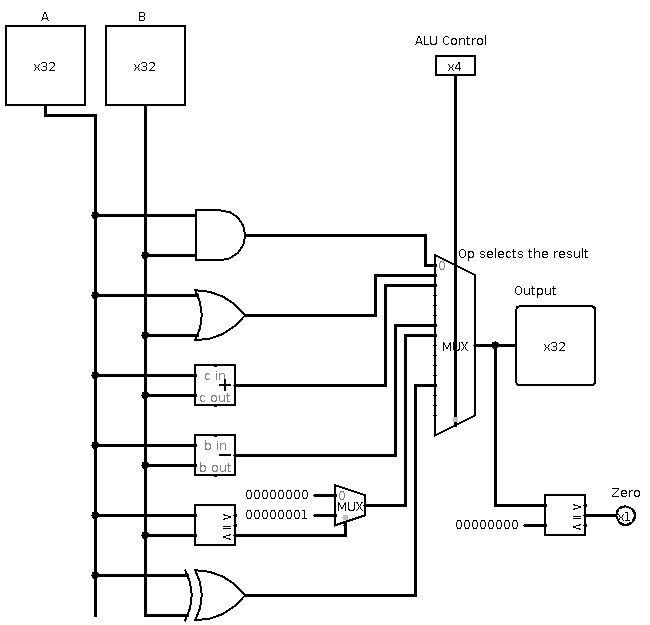
\includegraphics[width=300px]{./alu.png}
\caption{\label{fig:alu}
ALU.}
\end{figure}

\section{Decodificador de tipo}
\label{sec:org3245176}

Para saber qual tipo de instrução um opcode representa foi criado um decodificador de tipo para as instruções da tabela \ref{tab:procinstrucoes}. A figura \ref{fig:typedecode} mostra o esquemático.

\begin{figure}[htbp]
\centering
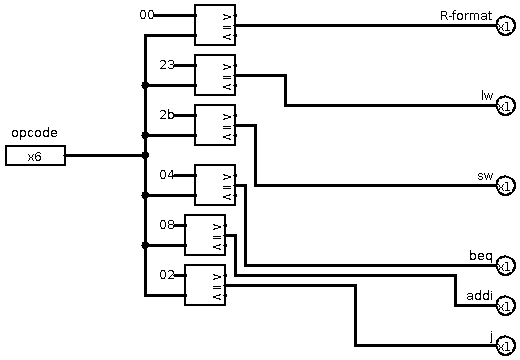
\includegraphics[width=.9\linewidth]{./typedecode.png}
\caption{\label{fig:typedecode}
Decodificador de tipo.}
\end{figure}


\section{Decodificador de controle}
\label{sec:orgc337f61}

Com o decodificador de tipo de instrução basta ativar os sinais de controle de acordo com a instrução de entrada. Essa decodificação para sinais de controle é feita de acordo com a tabela \ref{tab:controldecode}.(Sendo X um \emph{don't care})

A figura \ref{fig:controldecode} mostra o esquemático.

\begin{table}[htbp]
\centering
\begin{tabular}{l|c|c|c|c|c|c|}
 & R-format & lw & sw & beq & addi & j\\
\hline
RegDest & 1 & 0 & X & X & 0 & 0\\
AluSrc & 0 & 1 & 1 & 0 & 1 & 0\\
MemtoReg & 0 & 1 & X & X & 0 & 0\\
RegWrite & 1 & 1 & 0 & 0 & 1 & 0\\
MemRead & 0 & 1 & 0 & 0 & 0 & 0\\
MemWrite & 0 & 0 & 1 & 0 & 0 & 0\\
Branch & 0 & 0 & 0 & 1 & 0 & 0\\
ALUOp1 & 1 & 0 & 0 & 0 & 0 & 0\\
ALUOp0 & 0 & 0 & 0 & 1 & 0 & 0\\
Jump & 0 & 0 & 0 & 0 & 0 & 1\\
\end{tabular}
\caption{\label{tab:controldecode}
Sinais de controle de acordo com instrução.}

\end{table}

\begin{figure}[htbp]
\centering
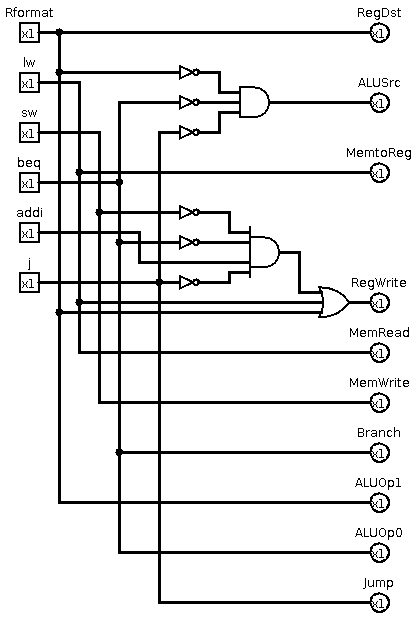
\includegraphics[width=300px]{./controldecode.png}
\caption{\label{fig:controldecode}
Decodificador de controle.}
\end{figure}

O addi tem AluSrc=1 para que o valor de [15..0](offset) da instrução seja somado ao valor do registrador, o RegWrite=1 é para que o valor seja escrito no registrador destino e o RegDst=0 para que o registrador que será escrito seja o [20..16](rt).(figura \ref{fig:itype})

\begin{figure}[htbp]
\centering
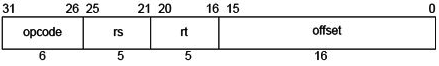
\includegraphics[width=230px]{./itype.png}
\caption{\label{fig:itype}
Instrução tipo I.}
\end{figure}

Para a instrução j foi criado um sinal de controle exclusivo chamado Jump que desencadeia as operações necessárias para que a instrução ocorra.

\section{Unidade de controle}
\label{sec:orgfd38917}

Com o decodificador de controle e decodificador de tipo basta juntá-los, o resultado disso é a figura \ref{fig:controlunit}.

\begin{figure}[htbp]
\centering
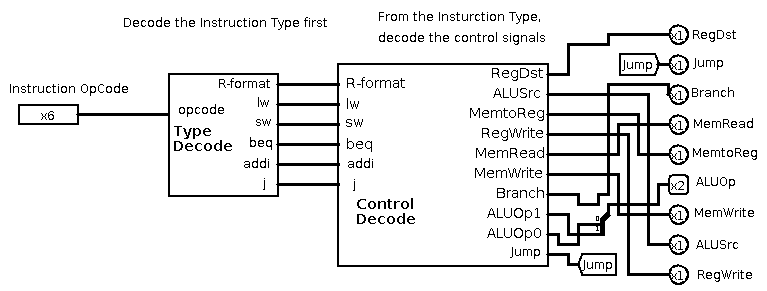
\includegraphics[width=.9\linewidth]{./controlunit.png}
\caption{\label{fig:controlunit}
Unidade de controle.}
\end{figure}

\section{Controle da ALU}
\label{sec:org9446161}

Cada tipo de instrução usa a ALU de alguma maneira diferente logo foi criado um controle de operações da ALU com base na tabela \ref{tab:controlalu}. Então de acordo com o campo funct da instrução e o sinal ALUOp o tipo de operação da ALU é escolhido. O esquemático do controle da ALU é dado na figura \ref{fig:controlalu}.

\begin{table}[htbp]
\centering
\begin{tabular}{|c|c|c|l}
ALUOp & Campo Funct & Operação & \\
\hline
00 & XXXXXX & 0010 & ADD\\
X1 & XXXXXX & 0110 & SUB\\
1X & XX0000 & 0010 & ADD\\
1X & XX0010 & 0110 & SUB\\
1X & XX0100 & 0000 & AND\\
1X & XX0101 & 0001 & OR\\
1X & XX1010 & 0111 & Set on less than\\
\hline
\end{tabular}
\caption{\label{tab:controlalu}
Controle da ALU.}

\end{table}

\begin{figure}[htbp]
\centering
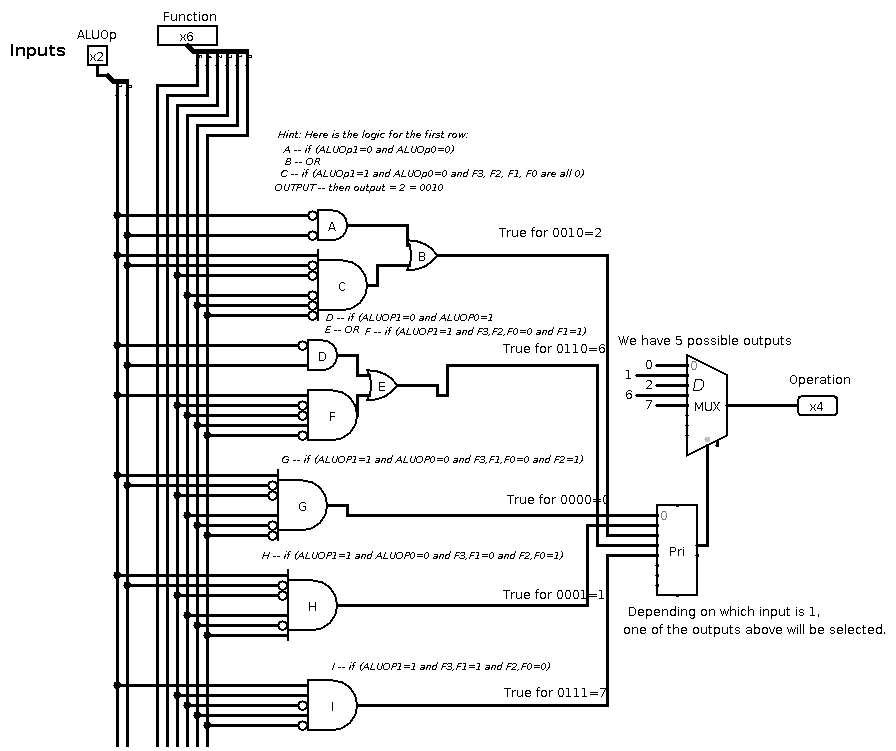
\includegraphics[width=330px]{./controlalu.png}
\caption{\label{fig:controlalu}
Controle da ALU.}
\end{figure}

\section{Caminho de dados}
\label{sec:org2a9f833}
O ultimo passo é a construção do caminho de dados. Na figura \ref{fig:mips} há o caminho de dados. É necessário interpretar as consequências de cada sinal de controle.

O RegDst controla qual registrador será escrito, será o endereço do registrador no campo rd se RegDst=1 ou o campo rt se RegDst=0.

Com RegWrite=1 o registrador que será escrito receberá os dados da entrada de escrita.

Com ALUSrc=0 o segundo operando da ALU será o segundo registrador lido. Já com ALUSrc=1 o segundo operando da ALU será os 16 bits de baixo da instrução atual([15:0]).

Com Branch=0 ou com os valores dos registradores diferentes o valor do PC(Program counter) será mudado para PC+4. Com Branch=1 e valores nos registradores iguais o valor de PC será substituído pelo offset da instrução deslocado 2 bits para a esquerda somado com o valor de PC+4. Porém se o Jump=1 então o valor de PC será substituído pelo valor obtido da lógica do Jump.

A lógica do Jump é de pegar os 26 bits do campo de imediato da instrução[25:0] e esses 26 bits com deslocamento de 2 para a esquerda serem a parte de [27:0] do endereço final e os 4 bits mais significativos de PC+4 serão a parte [31:28] do endereço final resultante.

Se MemRead=1 então com o endereço informado na entrada de endereço da memória é obtido o valor correspondente a esse endereço. Se MemWrite=1 então o conteúdo do endereço informado é substituído pelo valor na entrada de escrita da memória.

Se MemtoReg=0 então o valor indo para a entrada de dados de escrita do registrador vem da ALU, se não então o valor vem da memória.

As consequências do valor do ALUOp é descrito na tabela \ref{tab:controlalu}.


\begin{figure}[htbp]
\centering
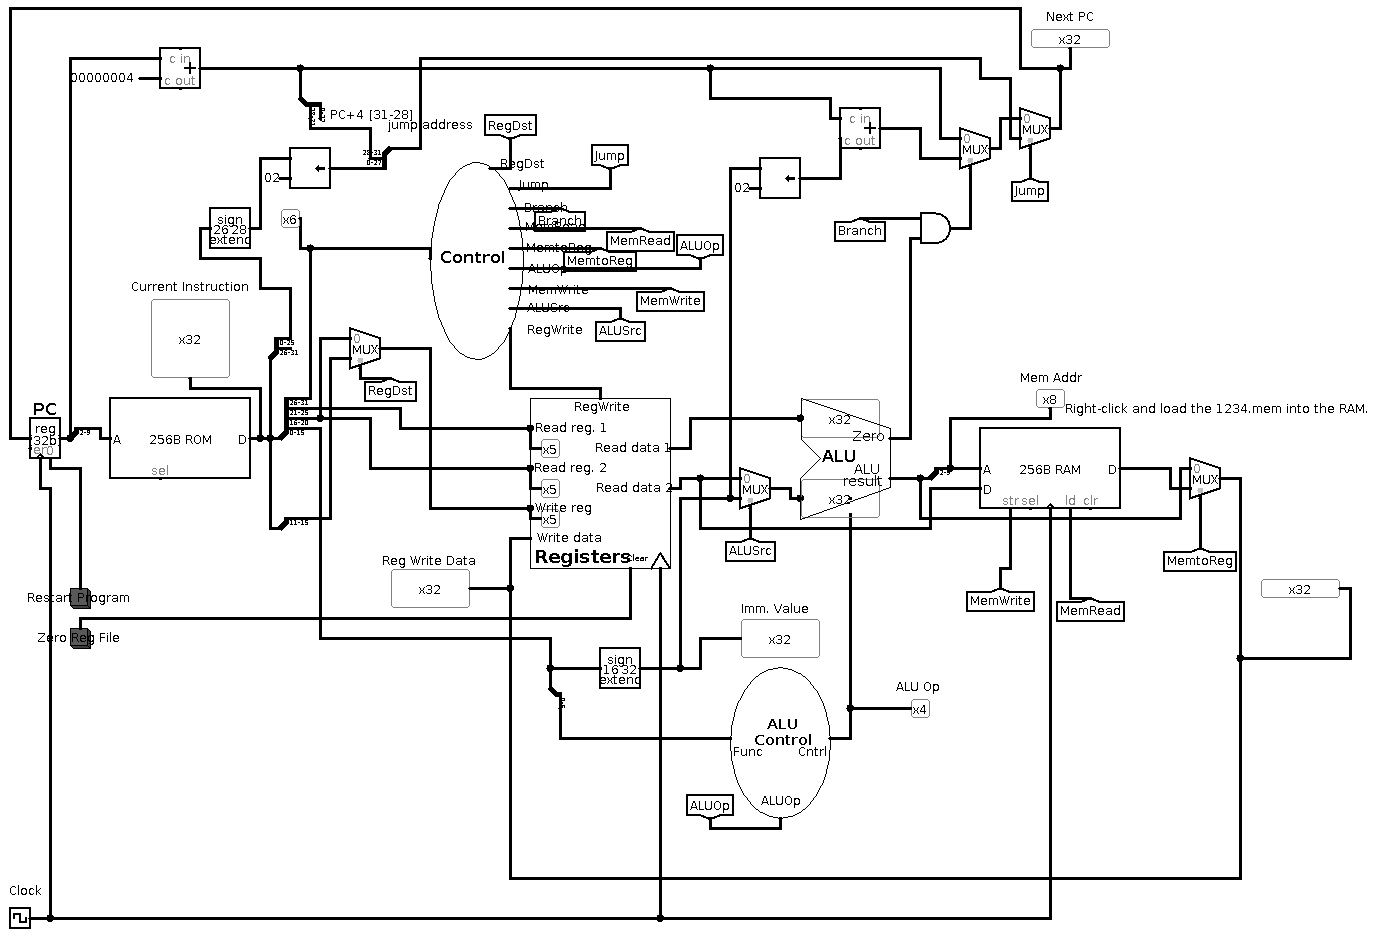
\includegraphics[width=450px]{./mips.png}
\caption{\label{fig:mips}
Caminho de dados.}
\end{figure}

\section{Validação}
\label{sec:orge619fae}

Para fazer a validação do processador criado foi utilizado o Mars 4.5 para fazer a transformação do código em assembly MIPS para hexadecimal. O código a seguir deve retornar a soma \(\sum_{i=1}^{a0}i\).

\begin{lstlisting}[language = mips]
lw $t0,0($zero)
# cumulative sum f(a0)
add $t1,$zero,$zero
sum_loop:
beq $t0,$zero,sum_exit
add $t1,$t1,$t0
addi $t0,$t0,-1
j sum_loop
sum_exit:
sw $t1,4($zero)
\end{lstlisting}


\begin{figure}[htbp]
\centering
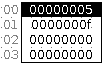
\includegraphics[width=100px]{./example1.png}
\caption{Exemplo de entrada e saída.(Entrada na primeira linha e saída na segunda)}
\end{figure}
\end{document}
